\documentclass[12pt,a4paper]{article}
\usepackage[utf8]{inputenc}
\usepackage[T1]{fontenc}
\usepackage[ngerman]{babel}
\usepackage{csquotes}
\usepackage[backend=biber,style=authoryear,maxcitenames=2,maxbibnames=99]{biblatex}
\addbibresource{Organisation.bib} % Bib-Datei nicht vergessen!
\newcommand{\zitat}[1]{\parencite{#1}}
\usepackage{geometry}
\geometry{
	left=30mm,
	right=30mm,
	top=25mm,
	bottom=25mm
}
\usepackage{graphicx}
\usepackage{float}
\usepackage{setspace}
\onehalfspacing
\usepackage{caption}
\usepackage{tocloft}
\usepackage{hyperref}
\hypersetup{colorlinks=true, linkcolor=black, urlcolor=blue, citecolor=black}
\usepackage{acronym}
\usepackage[nottoc]{tocbibind}
\usepackage{etoolbox} % für robusten Befehl
\usepackage{lipsum} % nur für Blindtext, kann entfernt werden
\usepackage{setspace} % für Zeilenabstand
\usepackage{ragged2e} % für \justifying





\newcommand{\absatzZitat}[1]{%
	\begin{quote}
		\fontsize{10pt}{12pt}\selectfont
		\setstretch{1.0}
		\leftskip=1cm
		\rightskip=1cm
		\justifying
		#1
	\end{quote}
}

\begin{document}
	
	%------------------------- Titelseite -------------------------
	\begin{titlepage}
		\centering
		\vfill
		{\Huge \textbf{Deutsche Telekom}}\\[1.5cm]
		\large
		Seminar: Grundlagen der Organisation\\
		Sommersemester 2025\\[2cm]
		
\includegraphics[width=0.4\textwidth]{images/UOL-Logo.png}\\[2cm]
		\normalsize
		\begin{flushleft}
			\textbf{Betreurin:} Prof. Dr. Julia Brennecke\\[0.5cm]
			\textbf{Abgegeben von:}\\
			Mika Scheinig\\
			Elija Wendte\\
			Justus Kressmann\\
			Engin Fidansoy\\
			Manar Krenbeh\\[0.5cm]
			Carl von Ossietzky Universität Oldenburg\\
			Fakultät II – Informatik, Wirtschafts- und Rechtswissenschaften\\
		\end{flushleft}
		\vfill
		\begin{flushright}
			Abgabedatum: 01. Juni 2025
		\end{flushright}
	\end{titlepage}
	
	%------------------------- Eidesstattliche Erklärung -------------------------
	\pagenumbering{Roman}
	
	\section*{\texorpdfstring{Executive Summary}{Executive Summary }}\label{executive-summary}
	
	In diesem Bericht wird die Aufbau- und Ablauforganisation der Deutschen
	Telekom AG untersucht, die mit rund 200.000 Mitarbeitenden in mehr als
	50 Ländern zu den größten Telekommunikationsanbietern weltweit gehört.
	Der Konzern organisiert sich im Wesentlichen divisional, wobei
	Matrixelemente in Bereichen wie IT, Personal und Strategie hinzukommen.
	Diese hybride Struktur soll Spezialisierung, Kund:innennähe und
	Flexibilität ermöglichen. Allerdings ergeben sich dabei auch
	Schwierigkeiten bei Koordination, Abstimmung und der Bestimmung
	eindeutiger Zuständigkeiten. Die Analyse legt offen, dass interne
	Abläufe teils als schwerfällig wahrgenommen werden.
	Entscheidungsprozesse nehmen viel Zeit in Anspruch, interdisziplinäre
	Kooperation funktioniert nicht optimal, und Silo-Denken erschwert eine
	übergreifende Sichtweise. Agile Arbeitsformen lassen sich unter diesen
	Bedingungen schwer integrieren. Bestehende Initiativen wie digitale
	Lernplattformen, neue Führungsmodelle und bereichsübergreifende Projekte
	sind wichtige Schritte, reichen jedoch nicht aus, um strukturelle
	Schwächen zu beheben.
	
	\noindent Der Schwerpunkt liegt auf der Geschäftseinheit T-Systems, bei der ein
	gesteigerter Veränderungsbedarf festgestellt wurde. Die Analyse zeigt
	Potenziale in Effizienz, Zuständigkeiten und Kulturentwicklung. Erste
	Handlungsideen wie klare Schnittstellen, effizientere Prozesse und
	vernetzte Zusammenarbeit werden skizziert. Der Bericht bildet die Basis
	für einen Folgebericht mit konkreten Empfehlungen zur Reorganisation von
	T-Systems.
	
	
	%------------------------- Inhaltsverzeichnis -------------------------
	\newpage
	\tableofcontents
	\newpage
	
	%------------------------- Abbildungsverzeichnis -------------------------
	\listoffigures
	\newpage
	
	%------------------------- Tabellenverzeichnis -------------------------
	\listoftables
	\newpage
	
	%------------------------- Abkürzungsverzeichnis -------------------------
	\section*{Abkürzungsverzeichnis}
	\begin{acronym}[IT]
		\acro{IT}{Informationstechnologie}
		\acro{BWL}{Betriebswirtschaftslehre}
	\end{acronym}
	\newpage
	
	%------------------------- Kapitelstruktur -------------------------
	
	\pagenumbering{arabic}
	\setcounter{page}{1}
	\begin{center}
		\textbf{Report 1 – Deutsche Telekom}
	\end{center}
	
	
	
	\section{Einleitung und Unternehmensvorstellung}
	
	\subsection{Kontext und Relevanz}
	Warum wurde diese Organisationseinheit gewählt?
	
	Einordnung in das Unternehmen (z.B. Bereich, Funktion, strategische Bedeutung)
	
	\subsection{ Überblick zur Organisationseinheit}
	Größe, Struktur, Aufgabenbereich
	
	Rolle innerhalb des Gesamtunternehmens
	\subsection{Kontext und Relevanz}
	Was soll mit dem Bericht erreicht werden?
	
	Kurze Vorschau auf den inhaltlichen Aufbau
	
	\subsection{Zielsetzung der Analyse}
	Was soll mit dem Bericht erreicht werden?
	
	Kurze Vorschau auf den inhaltlichen Aufbau
	
	
	\section{Analyse der informellen Organisation}
	\subsection{Informelle Strukturen und kulturelle Merkmale}
	Werte, Normen, interne Denkweisen
	
	Machtverhältnisse, Netzwerkstrukturen
	
	Informelle Kommunikation und Entscheidungswege
	\subsection{Elemente moderner Organisationsformen}
	Einsatz von agilen Methoden, selbstorganisierten Teams etc.
	
	Technologische Infrastruktur (z.B. Tools, Plattformen)
	
	Zusammenarbeit über Bereichsgrenzen hinweg (Cross-Functional Work)
	\subsection{Identifizierte Herausforderungen}
	
	Welche Spannungen oder Schwächen ergeben sich aus der Analyse?
	
	Konkrete Pain Points mit Bezug zur Organisationseinheit
	
	Bezug zur Risikoanalyse aus dem Geschäftsbericht
	
\section{Konzeptentwicklung für organisationalen Wandel}

\subsection{Ausgangspunkt und Problemfokus}

Wie in der Analyse gezeigt wurde, ist die eingeschränkte organisatorische Beweglichkeit ein zentrales Problem. Lange Entscheidungswege, fehlende Abstimmung zwischen Bereichen und eine geringe Reaktionsgeschwindigkeit erschweren die Zusammenarbeit und verringern die Innovationsfähigkeit der Organisation.

\noindent Das folgende Konzept greift dieses Problem direkt auf. Es verbindet technologische und organisatorische Ansätze, um Entscheidungswege zu verkürzen und Strukturen anpassungsfähiger zu machen. Im Mittelpunkt stehen vier zusammenhängende Bereiche: der Einsatz von Cloud- und SaaS-Technologien, der Ausbau datengestützter Entscheidungsunterstützung (BI), die Verbesserung bereichsübergreifender HR- und Wissensprozesse sowie die Einführung agiler Arbeitsformen. Die Maßnahmen orientieren sich an den im Geschäftsbericht 2021 genannten Risikofeldern und zielen auf eine Entscheidungsstruktur ab, die robust, flexibel und skalierbar ist.

\subsection{Zielsetzung des Konzepts}

Das Ziel des Konzepts ist es, die organisatorische Agilität in der betrachteten Organisationseinheit der Deutschen Telekom gezielt zu verbessern. Dafür sollen technologische, strukturelle und kulturelle Voraussetzungen geschaffen werden, die eine schnellere, abgestimmte und flexiblere Reaktion auf äußere Anforderungen ermöglichen.

\noindent Die Zielsetzung basiert auf dem in der strategischen Planung üblichen Aufbau aus Sach- und Formalzielen \parencite{StelzerDirk1962-2011I:GA}. Der Fokus liegt auf folgenden Punkten:

\begin{itemize}
	\item \textbf{Sachziel:} Die Organisation soll besser auf regulatorische, technologische und marktbedingte Veränderungen reagieren können – durch gezielten Einsatz agiler Methoden, cloudbasierter Systeme und strukturierter Wissensprozesse.
	\item \textbf{Formalziele:} Bessere Wirksamkeit durch zentrale Entscheidungen und BI-Transparenz, mehr Anpassungsfähigkeit durch flexible SaaS-Workflows und Teams, sowie durch systematische Nutzung und schrittweise Einführung.
\end{itemize}

\subsection{Zielsystem}\label{sec:zielsystem}

\begin{itemize}
	\item \textbf{Ziel 1:} Innerhalb eines Jahres soll die durchschnittliche Dauer bereichsübergreifender Entscheidungsprozesse um mindestens 30\,\% gesenkt werden. Gemessen wird die Zeit zwischen Start und Umsetzung (KPI: Entscheidungsdurchlaufzeit).
	
	\item \textbf{Ziel 2:} Die Zustimmung zur Aussage „Veränderungen werden nachvollziehbar kommuniziert“ soll nach sechs Monaten bei mindestens 75\,\% liegen. Erfasst wird dies über eine interne Zufriedenheitsumfrage (KPI: Change-Kommunikationsfeedback).
\end{itemize}

\subsection{Konzeptionelle Ansätze und Maßnahmen}

\subsubsection{Ansatz 1}
Integriertes Konzept für agile Entscheidungsunterstützung: Kombination von Business Intelligence und SaaS.

\paragraph{1. BI-basierte Entscheidungsunterstützung: Daten als Grundlage}

Laut Smith und Ariyachandra (2021) kann eine einfache, aber gut strukturierte BI-Lösung Entscheidungsprozesse deutlich verbessern. In ihrer Analyse der FEMA-Studie betonen sie:

\begin{quote}
	A simple integrated BI solution [...] can vastly enhance the post disaster operations [...] and improve its agility during humanitarian crises. \parencite[210]{rahman_achieving_2022}.
\end{quote} 

\noindent Die dort beschriebenen Probleme – wie fehlende Transparenz, lange Entscheidungswege oder unklare Zuständigkeiten – sind in ähnlicher Form auch bei der Deutschen Telekom zu erkennen.

\noindent Um das gezielt zu verbessern, bietet sich ein strukturiertes Vorgehen auf Basis folgender fünf Punkte an:

\begin{itemize}
	\item \textbf{Datenerfassung und -bereinigung:} Im Mittelpunkt stehen operative Daten aus Telekom-Systemen – etwa zu Projekten, IT-Tickets oder Personaleinsätzen. Diese sollen automatisch geprüft und zusammengeführt werden, um bessere Entscheidungsgrundlagen zu schaffen. Denn: „Data accuracy and data completeness are […] key problems“ \parencite[S.~201]{rahman_achieving_2022}.
	
	\item \textbf{Zentrale Datenintegration:} Aufbau eines cloudbasierten, einheitlichen Datenmodells mit klaren Schnittstellen zwischen Bereichen.
	
	\item \textbf{Rollenbasiertes Echtzeit-Reporting:} Dashboards zeigen je nach Rolle Kennzahlen zu Entscheidungsdauer, Rückläufen und Beteiligung.
	
	\item \textbf{Governance-Struktur:} Klare Zuständigkeiten für Datenqualität, Reporting und KPI-Management.
	
	\item \textbf{Pilotierung:} Start mit agilen, interdisziplinären Teams zur schrittweisen Einführung und zur Förderung der Akzeptanz.
\end{itemize}

\noindent Ziel ist es, Entscheidungen transparenter, schneller und datenbasiert zu machen – das ist ein wichtiger Schritt, um die Agilität im Unternehmen zu steigern.

\paragraph{2. SaaS-basierte Entscheidungsstrukturen: Prozesse flexibler gestalten}

Business Intelligence (BI) sorgt für bessere Entscheidungsgrundlagen. Der SaaS-Ansatz (Software-as-a-Service) geht einen Schritt weiter: Er macht die Entscheidungsprozesse selbst flexibler, transparenter und technisch besser skalierbar. Für ein Unternehmen wie die Deutsche Telekom bedeutet das, Entscheidungswege zu vereinfachen, Zuständigkeiten klarer zu regeln und Prozesse dynamisch anzupassen.

\noindent Entscheidungsstrukturen lassen sich als digitale Services abbilden – mit klaren Schnittstellen, automatischem Feedback und standardisierter Überwachung. Cloudbasiertes Wissensmanagement kann die nötige Beweglichkeit schaffen, um qualitativ gute Entscheidungen zu ermöglichen \parencite{churakova2010software}.

\noindent Die Einführung erfolgt idealerweise schrittweise nach einem angepassten Modell von Chou und Chou (2011), das sich auf die Arbeiten von \parencite{murthy2010tapping}, \parencite{chong2006multi} und \parencite{buyya2008market} stützt. Das Modell besteht aus sechs aufeinander aufbauenden Phasen und wurde für große Organisationen wie die Telekom angepasst (vgl. Abbildung~\ref{fig:saas-implementation-plan}).

\begin{figure}[H]
	\centering
	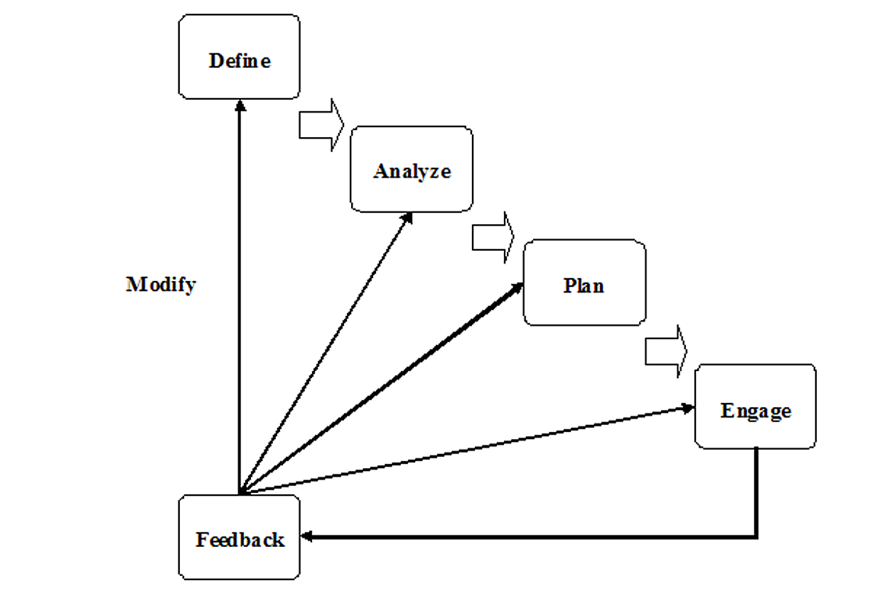
\includegraphics[width=0.6\textwidth]{./images/saas_implementation_plan.png}
	\caption{Modifizierter SaaS-Implementierungsplan nach \textcite{chou2011cloud}, basierend auf \textcite{murthy2010tapping}, \textcite{chong2006multi} und \textcite{buyya2008market}}
	\label{fig:saas-implementation-plan}
\end{figure}

\begin{itemize}
	\item \textbf{Define:} Zuerst wird festgehalten, wo es aktuell Probleme gibt – zum Beispiel Medienbrüche, unklare Zuständigkeiten oder isolierte Systeme.
	
	\item \textbf{Analyze:} Danach wird die IT-Struktur analysiert, die Ziele der Fachbereiche aufgenommen und mögliche Hürden bei der Integration betrachtet.
	
	\item \textbf{Plan:} Auf dieser Grundlage wird die Migration zu SaaS geplant. Dazu gehören die Auswahl von Anbietern, technische Anforderungen und rechtliche Rahmenbedingungen (z.\,B. Datenschutz, SLAs).
	
	\item \textbf{Engage:} Die Umsetzung beginnt klein – zum Beispiel in einem Bereich mit vielen Abstimmungen – um erste Erfahrungen zu sammeln und direkt nachzubessern.
	
	\item \textbf{Feedback:} Erste Umsetzungsschritte werden laufend bewertet – zum Beispiel in Bezug auf Bedienbarkeit, Schnittstellen oder die Akzeptanz bei den Mitarbeitenden.
	
	\item \textbf{Modify:} Auf Basis des Feedbacks werden technische und organisatorische Anpassungen gemacht. Ziel ist eine Lösung, die passt und sich skalieren lässt.
\end{itemize}

\noindent Die Telekom kann mit diesem Ansatz Entscheidungsprozesse serviceorientiert, nachvollziehbar und flexibel gestalten. Damit werden auch die definierten Formalziele unterstützt: Softwaregestützte Strukturen erhöhen die Wirksamkeit, konfigurierbare Workflows steigern die Anpassungsfähigkeit, und zentral verfügbare Dienste verbessern die Effizienz – auch über Bereichsgrenzen hinweg.

\noindent Die Verbindung von BI (für bessere Entscheidungsinhalte) und SaaS (für flexible Prozesse) ergibt ein durchdachtes Gesamtkonzept, das direkt zur Stärkung der organisatorischen Beweglichkeit beiträgt – eine praxisnahe Antwort auf die Herausforderungen der Konzernsteuerung.

\subsubsection{Ansatz 2}

\paragraph{Kontextuelle Ambidexterität als Kulturansatz zur Verbesserung der Change-Kommunikation}

Neben technologischen Maßnahmen braucht es auch eine passende Unternehmenskultur, um echte Beweglichkeit zu erreichen. Ein sinnvoller Ansatz ist die sogenannte kontextuelle Ambidexterität. Dabei geht es darum, Mitarbeitende in die Lage zu versetzen, eigenständig zwischen effizientem Arbeiten (Exploitation) und dem Erkunden neuer Lösungen (Exploration) zu wechseln. Es wird also nicht auf starre Strukturen oder einzelne Führungspersonen gesetzt, sondern ein Umfeld geschaffen, das auf Eigenverantwortung und Anpassungsfähigkeit setzt.

\noindent\textcite{kumkale_organizational_2022} beschreiben das als „Führung durch Kontext“:

\begin{quote}
	Ambidexterity does not come into view from the formal structure alone or the vision statements of a charismatic leader, but rather requires the creation of a supportive context in which individuals make their own choices about how and where to focus their energies. \parencite[18]{kumkale_organizational_2022}.
\end{quote}

\noindent Für die Telekom heißt das, Rahmenbedingungen zu schaffen, damit auf allen Ebenen Führungsverantwortung übernommen werden kann – besonders in Zeiten des Wandels. Dazu gehören:

\begin{itemize}
	\item ein klar formulierter Handlungsrahmen (Alignment),
	\item die aktive Einbindung der Mitarbeitenden in Entscheidungen (Empowerment),
	\item und eine Feedbackkultur, die Lernen und Anpassung ermöglicht (Adaptability).
\end{itemize}

\noindent Ziel ist es, die Zustimmung zur Aussage „Veränderungen werden nachvollziehbar kommuniziert“ dauerhaft zu steigern (vgl. Ziel 2 in Abschnitt~\ref{sec:zielsystem}). Mehr Eigenverantwortung und Orientierung im Arbeitsalltag fördern nicht nur das Verständnis für Veränderungen, sondern verbessern auch die Umsetzung selbst.

	
	\section{Diskussion der Ergebnisse}
		\subsection{Umgang mit potenziellen Widerständen}
	Bezug auf bekannte Widerstandsursachen (vgl. Abbildung)
	
	Maßnahmen zur Förderung der Akzeptanz:
	
	Partizipation
	
	Change Agents
	
	Kommunikation und Transparenz
	
	Weiterbildung
	
	Ziel: Konzept so gestalten, dass es nicht gegen, sondern mit den Mitarbeitenden umgesetzt wird
	
	\subsection{Voraussetzungen und Erfolgsfaktoren}
	Was braucht es, damit das Konzept funktioniert?
	→ z.B. Unterstützung durch Führung, Ressourcen, Pilotbereiche
	
	Verbindung zu bestehenden Initiativen in der Organisation (z.B. Tech  Innovation bei der Telekom)
	\subsection{Bewertung der vorgeschlagenen Maßnahmen}
	
	Was leisten die Maßnahmen im Hinblick auf die analysierten Probleme?
	Welche Verbesserungen wären zu erwarten?
	\subsection{Potenziale und Chancen}
	Welche Entwicklungsmöglichkeiten ergeben sich für die Organisationseinheit?
	
	Langfristiger Nutzen (z.B. Innovationskraft, Arbeitgeberattraktivität)
	\subsection{Risiken und Grenzen}
	Was könnte die Umsetzung erschweren? (z.B. Ressourcen, Akzeptanz, Führung)
	
	Wo stößt das Konzept an Grenzen?
	
	\subsection{Einschätzung zur Umsetzbarkeit}
	Was spricht für die praktische Umsetzung?
	
	Welche Voraussetzungen müssen erfüllt sein?
	%------------------------- Literaturverzeichnis -------------------------
	
	\newpage
	\pagenumbering{roman}
	\printbibliography[heading=bibintoc,title={Literaturverzeichnis}]
	
	
	%------------------------- unternehmensinfo -------------------------
	\newpage
	\thispagestyle{empty} % keine Seitenzahl anzeigen
	\begin{figure}[H]
		\centering
		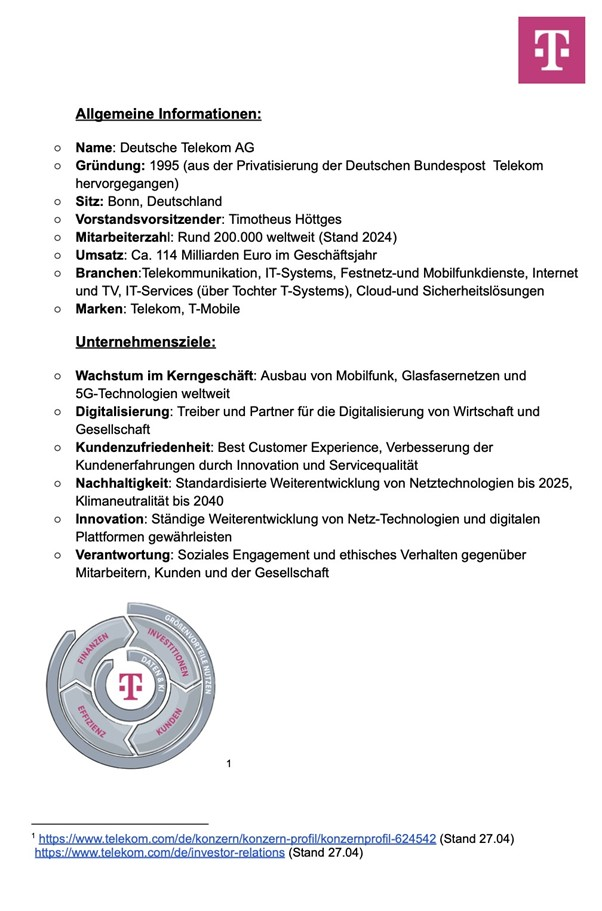
\includegraphics{images/Bild1.jpg}
	\end{figure}
	\newpage
	%------------------------- Anhang -------------------------
	\newpage
	\section{Anhang}
	[Zusätzliche Materialien wie Interviewleitfäden etc.]
	
	%------------------------- KI-Nutzung -------------------------
	\newpage
	\section{Anhang: Nutzung von Künstlicher Intelligenz}
	\begin{itemize}
		\item \textbf{Tool:} ChatGPT
		\item \textbf{URL:} \url{https://chatgpt.com}
		\item \textbf{Prompt:} „Erstelle eine vollständige LaTeX-Vorlage für eine Gruppenarbeit.“
		\item \textbf{Verwendet durch:} Manar Krenbeh
		\item \textbf{Datum:} 04.07.2025
	\end{itemize}
	\begin{itemize}
		\item \textbf{URL:} \url{https://chatgpt.com/share/682f2a68-37b8-8007-9855-d878bcd54ae3}
		\item \textbf{Prompt:} „Kannst du mir ein konkretes Beispiel für einen überregulierten internen Prozess der Deutschen Telekom nennen?“
		\item \textbf{Verwendet durch:} Mika Scheinig
		\item \textbf{Datum:} 22.05.2025
	\end{itemize}
	
	\begin{itemize}
		\item \textbf{URL:} \url{https://chatgpt.com/c/683721e2-4a9c-8001-b0a1-f2e5a1b3f5f2}
		\item \textbf{Prompt:} „Bitte erläutere die Unterschiede in der Leitungsspanne zwischen standardisierten operativen Bereichen und komplexeren Organisationseinheiten wie der Matrixorganisation bei T-Systems. Wie beeinflusst die Organisationsstruktur die Anzahl der direkt unterstellten Mitarbeitenden, und welche Herausforderungen ergeben sich für Führungskräfte in einer Matrixstruktur?“
		\item \textbf{Verwendet durch:} Justus Kressmann
		\item \textbf{Datum:} 24.05.2025
		\item \textbf{Tool:} NoteBook
		\item \textbf{URL:} \url{https://notebooklm.google.com}
		\item \textbf{Prompt:} "Finde aus dem Buch konkrete Methoden, wie Informationssysteme genutzt werden können, um Entscheidungsprozesse in Organisationen zu beschleunigen oder transparenter zu machen. Bitte nenne die jeweiligen Kapitel oder Autorenbeiträge." Hier \parencite{StelzerDirk1962-2011I:GA} verwendet
		\item \textbf{Verwendet durch:} Manar Krenbeh
		\item \textbf{Datum:} 05.07.2025
		\item \textbf{Prompt:} "Suche im Buch nach alternativen Lösungsansätzen oder Methoden zur Verbesserung der internen Kommunikation von Veränderungen im Unternehmen – ohne Bezug auf SaaS oder Business Intelligence." Hier \parencite{kumkale_organizational_2022} verwendet
		\item \textbf{Verwendet durch:} Manar Krenbeh
		\item \textbf{Datum:} 05.07.2025
	\end{itemize}
	
	\newpage
	\section*{Eidesstattliche Erklärung}
	Hiermit versichern wir, dass wir die vorliegende Arbeit selbstständig und nur mit den angegebenen Hilfsmitteln und Quellen angefertigt haben. Alle Stellen, die wörtlich oder sinngemäß aus Quellen übernommen wurden, sind entsprechend kenntlich gemacht. Die Arbeit wurde in gemeinsamer Verantwortung erstellt.
	
	\vspace{2cm}
	Oldenburg, 01. Juni 2025
	
	Unterschriften: \\
	\rule{5cm}{0.4pt} Mika Scheinig \\
	\rule{5cm}{0.4pt} Elija Wendte \\
	\rule{5cm}{0.4pt} Justus Kressmann \\
	\rule{5cm}{0.4pt} Engin Fidansoy \\
	\rule{5cm}{0.4pt} Manar Krenbeh
	
\end{document}
